\documentclass{beamer}
\usepackage[utf8]{inputenc}

\usetheme{Madrid}
\usecolortheme{default}
\usepackage{amsmath,amssymb,amsfonts,amsthm}
\usepackage{txfonts}
\usepackage{tkz-euclide}
\usepackage{listings}
\usepackage{adjustbox}
\usepackage{array}
\usepackage{tabularx}
\usepackage{gvv}
\usepackage{lmodern}
\usepackage{circuitikz}
\usepackage{tikz}
\usepackage{graphicx}

\setbeamertemplate{page number in head/foot}[totalframenumber]

\usepackage{tcolorbox}
\tcbuselibrary{minted,breakable,xparse,skins}



\definecolor{bg}{gray}{0.95}
\DeclareTCBListing{mintedbox}{O{}m!O{}}{%
  breakable=true,
  listing engine=minted,
  listing only,
  minted language=#2,
  minted style=default,
  minted options={%
    linenos,
    gobble=0,
    breaklines=true,
    breakafter=,,
    fontsize=\small,
    numbersep=8pt,
    #1},
  boxsep=0pt,
  left skip=0pt,
  right skip=0pt,
  left=25pt,
  right=0pt,
  top=3pt,
  bottom=3pt,
  arc=5pt,
  leftrule=0pt,
  rightrule=0pt,
  bottomrule=2pt,
  toprule=2pt,
  colback=bg,
  colframe=orange!70,
  enhanced,
  overlay={%
    \begin{tcbclipinterior}
    \fill[orange!20!white] (frame.south west) rectangle ([xshift=20pt]frame.north west);
    \end{tcbclipinterior}},
  #3,
}
\lstset{
    language=C,
    basicstyle=\ttfamily\small,
    keywordstyle=\color{blue},
    stringstyle=\color{orange},
    commentstyle=\color{green!60!black},
    numbers=left,
    numberstyle=\tiny\color{gray},
    breaklines=true,
    showstringspaces=false,
}
%------------------------------------------------------------

\title
{8.2.37}
\date{September 18, 2025}
\author 
{AI25BTECH11003 - Bhavesh Gaikwad}



\begin{document}


\frame{\titlepage}
\begin{frame}{Question}
Find the equation of the conic, that satisfies the given conditions.
vertex (-3, 0), directrix x + 5 = 0.
\end{frame}


\begin{frame}[fragile]
    \frametitle{Theoretical Solution}
Given:
\begin{itemize}
\item Vertex: $\vec{V} = \myvec{-3 \\ 0}$
\item Directrix: $x + 5 = 0$, which gives us $\vec{n}^\top\vec{x} = c$ where $\vec{n} = \myvec{1 \\ 0}$ and $c = -5$
\end{itemize}

The general matrix equation of a conic is:
\begin{equation}
\vec{x}^\top\vec{V}\vec{x} + 2\vec{u}^\top\vec{x} + f = 0
\end{equation}

where the matrices are defined as:
\begin{align}
\vec{V} &= \norm{\vec{n}}^2\vec{I} - e^2(\vec{n}\vec{n}^\top) \\
\vec{u} &= (ce^2)\vec{n} - \norm{\vec{n}}^2\vec{F} \\
f &= \norm{\vec{n}}^2\norm{\vec{F}}^2 - c^2e^2
\end{align}
\end{frame}


\begin{frame}[fragile]
    \frametitle{Theoretical Solution}
For a vertex at $(-3, 0)$ and using the vertex-focus-directrix geometry, the focus $\vec{F}$ is at:
\begin{equation}
\vec{F} = \myvec{-3 + 2e \\ 0}
\end{equation}

\newpage

\textbf{Case 1: $e < 1$} (Ellipse)\\
Let $e = \frac{1}{2}$

\textbf{Parameters:}
\begin{itemize}
\item $\vec{n} = \myvec{1 \\ 0}$, $c = -5$, $e = \frac{1}{2}$
\item $\vec{F} = \myvec{-2 \\ 0}$
\item $\norm{\vec{n}}^2 = 1$, $\norm{\vec{F}}^2 = 4$
\end{itemize}
\end{frame}


\begin{frame}[fragile]
    \frametitle{Theoretical Solution}
Matrix Calculation:
\begin{align}
\vec{V} &= \myvec{1 & 0 \\ 0 & 1} - \frac{1}{4}\myvec{1 & 0 \\ 0 & 0} = \myvec{3/4 & 0 \\ 0 & 1}
\end{align}

\begin{align}
\vec{u} &= \frac{-5}{4}\myvec{1 \\ 0} - \myvec{-2 \\ 0} = \myvec{3/4 \\ 0}
\end{align}

\begin{align}
f &= 4 - \frac{25}{4} = -\frac{9}{4}
\end{align}

Putting Values of $\vec{V}, \, \vec{u}$, f in Equation 0.1, we get
\begin{equation}
\vec{x}^\top\myvec{3 & 0 \\ 0 & 4}\vec{x} + \myvec{6 & 0}\vec{x} = 9
\end{equation}

\end{frame}



\begin{frame}[fragile]
    \frametitle{Theoretical Solution}
\textbf{Case 2: $e = 1$} (Parabola)\\
\textbf{Parameters:}
\begin{itemize}
\item $\vec{n} = \myvec{1 \\ 0}$, $c = -5$, $e = 1$
\item $\vec{F} = \myvec{-1 \\ 0}$
\item $\norm{\vec{F}}^2 = 1$
\end{itemize}

Matrix Calculation:
\begin{align}
\vec{V} &= \myvec{1 & 0 \\ 0 & 1} - \myvec{1 & 0 \\ 0 & 0} = \myvec{0 & 0 \\ 0 & 1}
\end{align}

\begin{align}
\vec{u} &= -5\myvec{1 \\ 0} - \myvec{-1 \\ 0} = \myvec{-4 \\ 0}
\end{align}

\begin{align}
f &= 1 - 25 = -24
\end{align}
\end{frame}

\begin{frame}[fragile]
    \frametitle{Theoretical Solution}
Putting Values of $\vec{V}, \, \vec{u}$, f in Equation 1, we get
\begin{equation}
\vec{x}^\top\myvec{0 & 0 \\ 0 & 1}\vec{x} + \myvec{-8 & 0}\vec{x} = 24
\end{equation}
\end{frame}

\begin{frame}[fragile]
    \frametitle{Theoretical Solution}
    \textbf{Case 3: $e > 1$} (Hyperbola)\\
Let $e = \frac{3}{2}$

\textbf{Parameters:}
\begin{itemize}
\item $\vec{n} = \myvec{1 \\ 0}$, $c = -5$, $e = \frac{3}{2}$
\item $\vec{F} = \myvec{0 \\ 0}$
\item $\norm{\vec{F}}^2 = 0$
\end{itemize}
Matrix Calculation:
\begin{align}
\vec{V} &= \myvec{1 & 0 \\ 0 & 1} - \frac{9}{4}\myvec{1 & 0 \\ 0 & 0} = \myvec{-5/4 & 0 \\ 0 & 1}
\end{align}

\begin{align}
\vec{u} &= \frac{-45}{4}\myvec{1 \\ 0} - \myvec{0 \\ 0} = \myvec{-45/4 \\ 0}
\end{align}
\end{frame}

\begin{frame}[fragile]
    \frametitle{Theoretical Solution}
\begin{align}
f &= 0 - \frac{225}{4} = -\frac{225}{4}
\end{align}

Putting Values of $\vec{V}, \, \vec{u}$, f in Equation 1, we get
\begin{equation}
\vec{x}^\top\myvec{5 & 0 \\ 0 & -4}\vec{x} + \myvec{90 & 0}\vec{x} + 225 = 0
\end{equation}

\end{frame}


\begin{frame}[fragile]
    \frametitle{Theoretical Solution}
Therefore, The Possible conics with the vertex at (-3,0) and Directrix as x+5=0 are\\
\begin{itemize}
\item$\vec{x}^\top\myvec{3 & 0 \\ 0 & 4}\vec{x} + \myvec{6 & 0}\vec{x} = 9$
\item$\vec{x}^\top\myvec{0 & 0 \\ 0 & 1}\vec{x} + \myvec{-8 & 0}\vec{x} = 24$
\item$\vec{x}^\top\myvec{5 & 0 \\ 0 & -4}\vec{x} + \myvec{90 & 0}\vec{x} + 225 = 0$
\end{itemize}
\end{frame}


\begin{frame}{Ellipse}
\begin{figure}
   \centering
    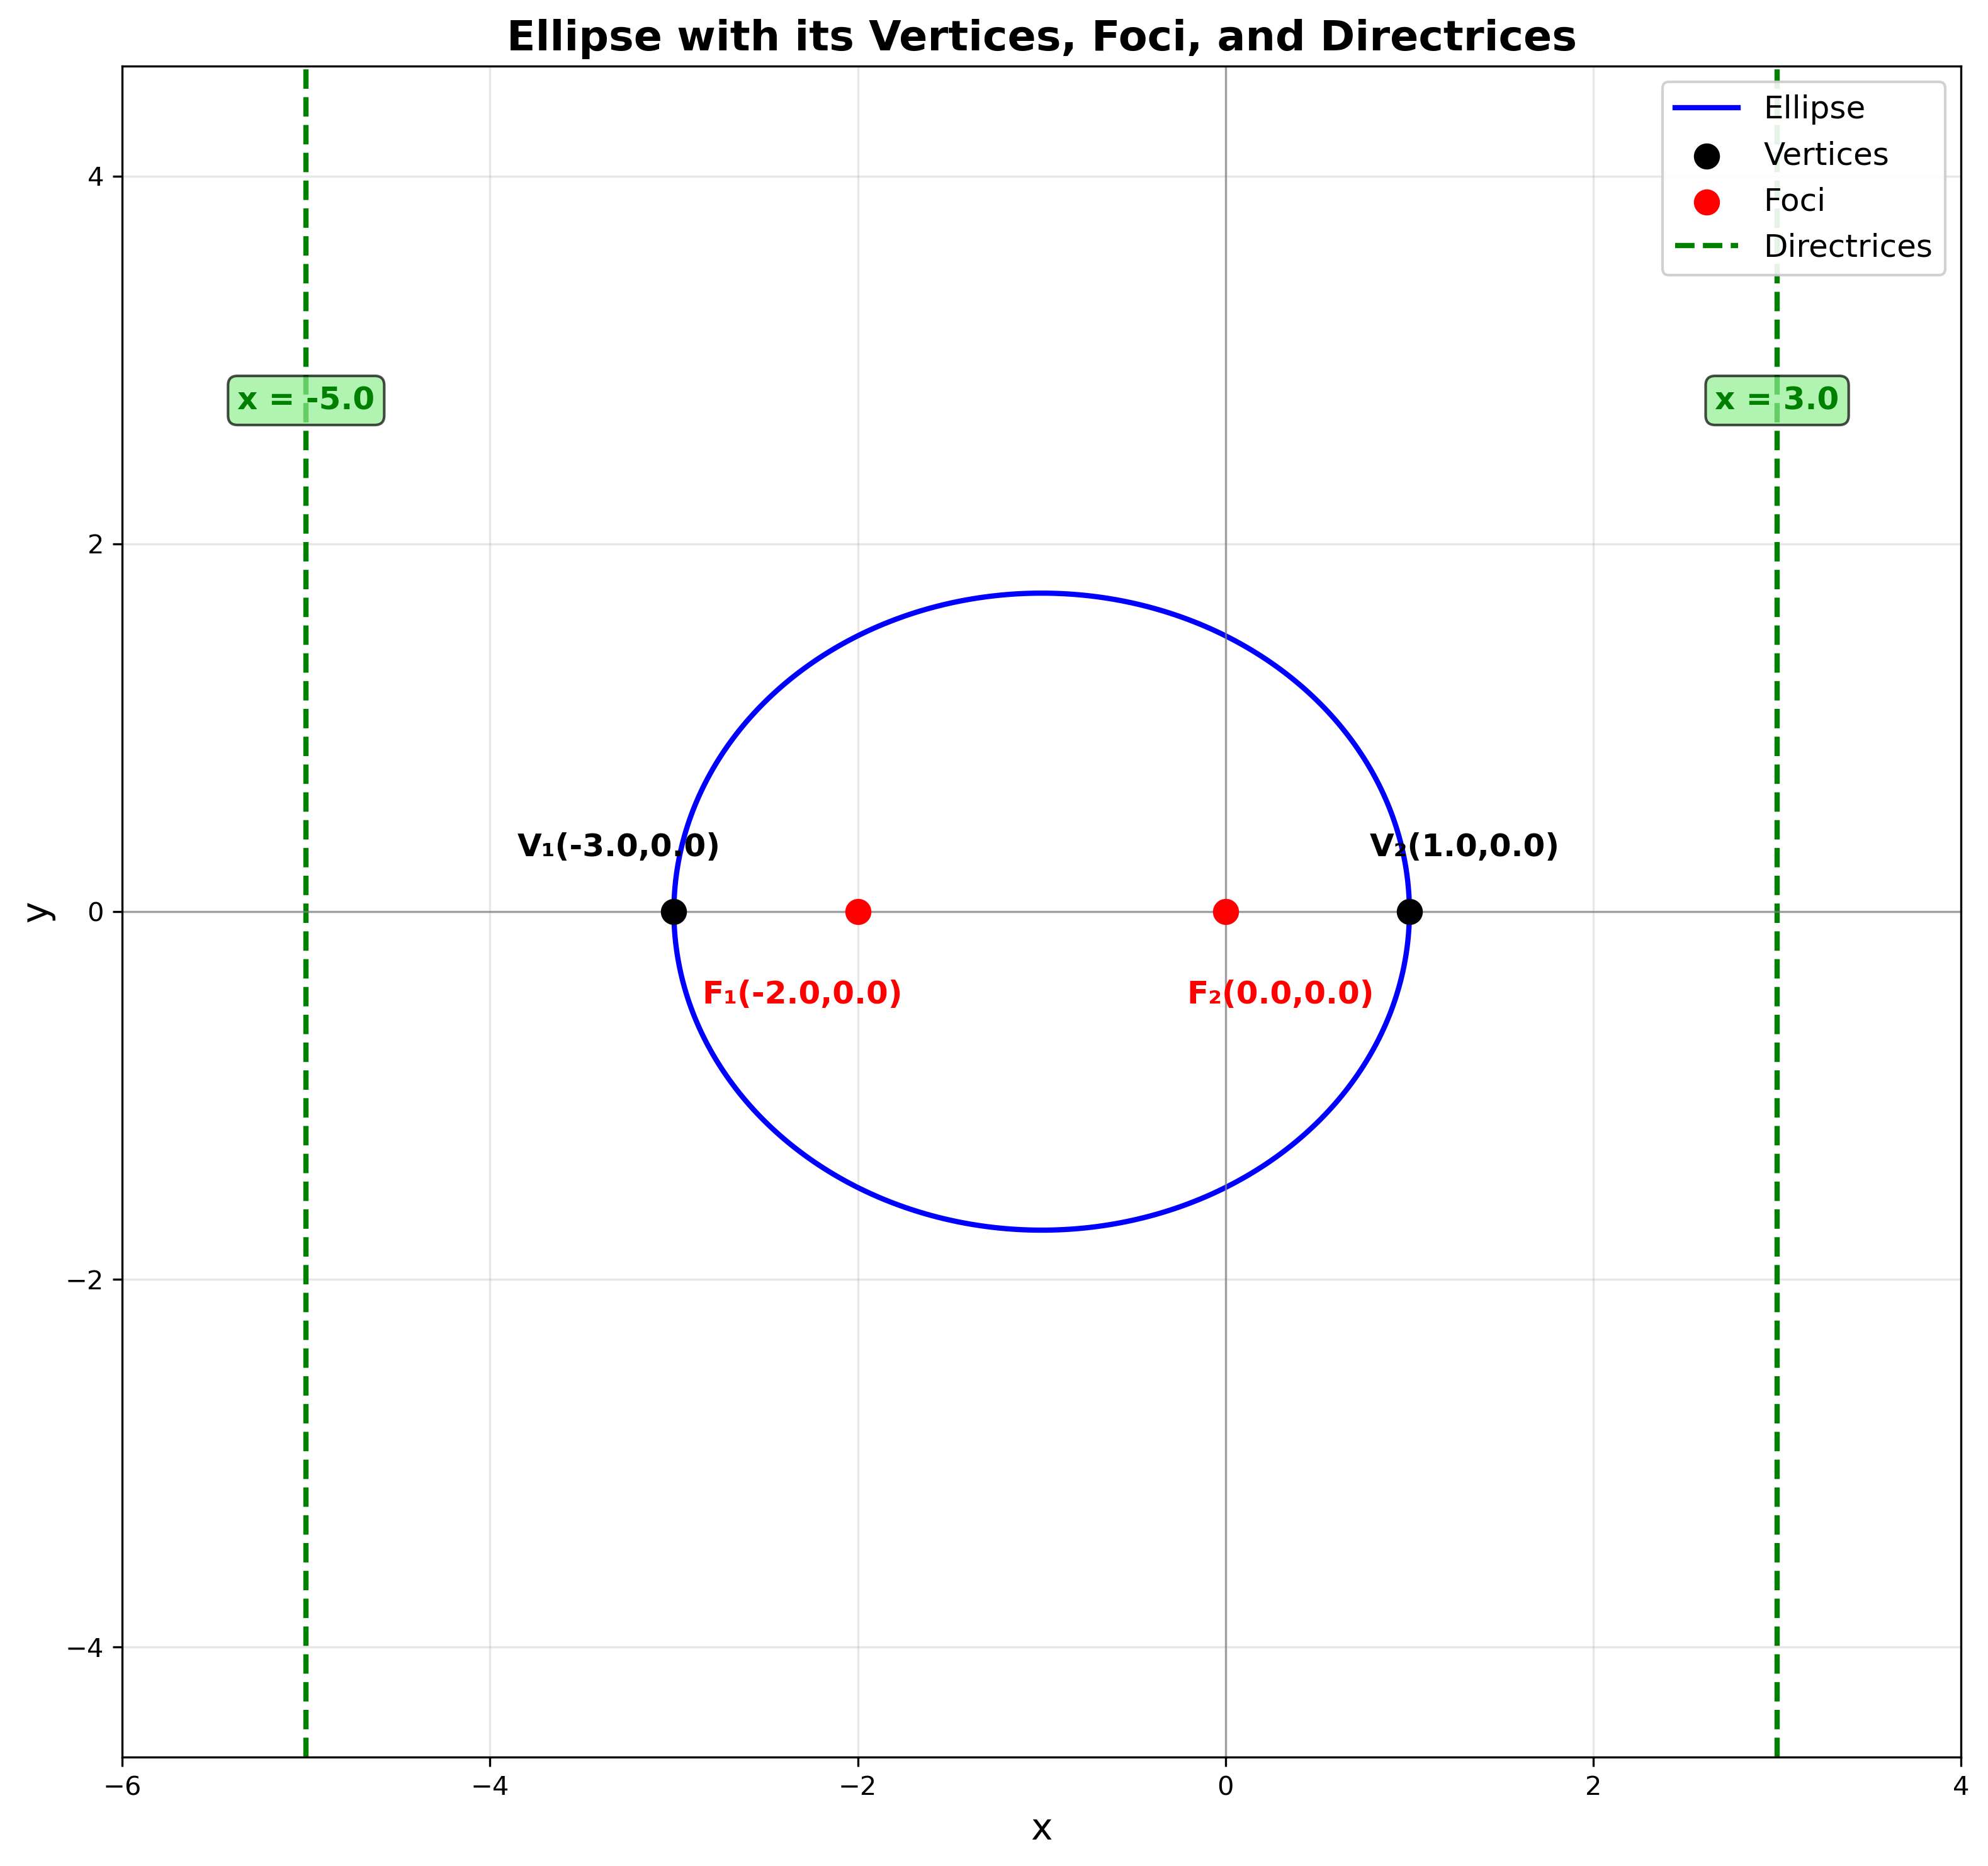
\includegraphics[width=\columnwidth, height=0.8\textheight, keepaspectratio]{figs/fig1.png}
    \label{fig:Beamer/figs/fig1.png}
\end{figure}
\end{frame}

\begin{frame}{Parabola}
\begin{figure}
   \centering
    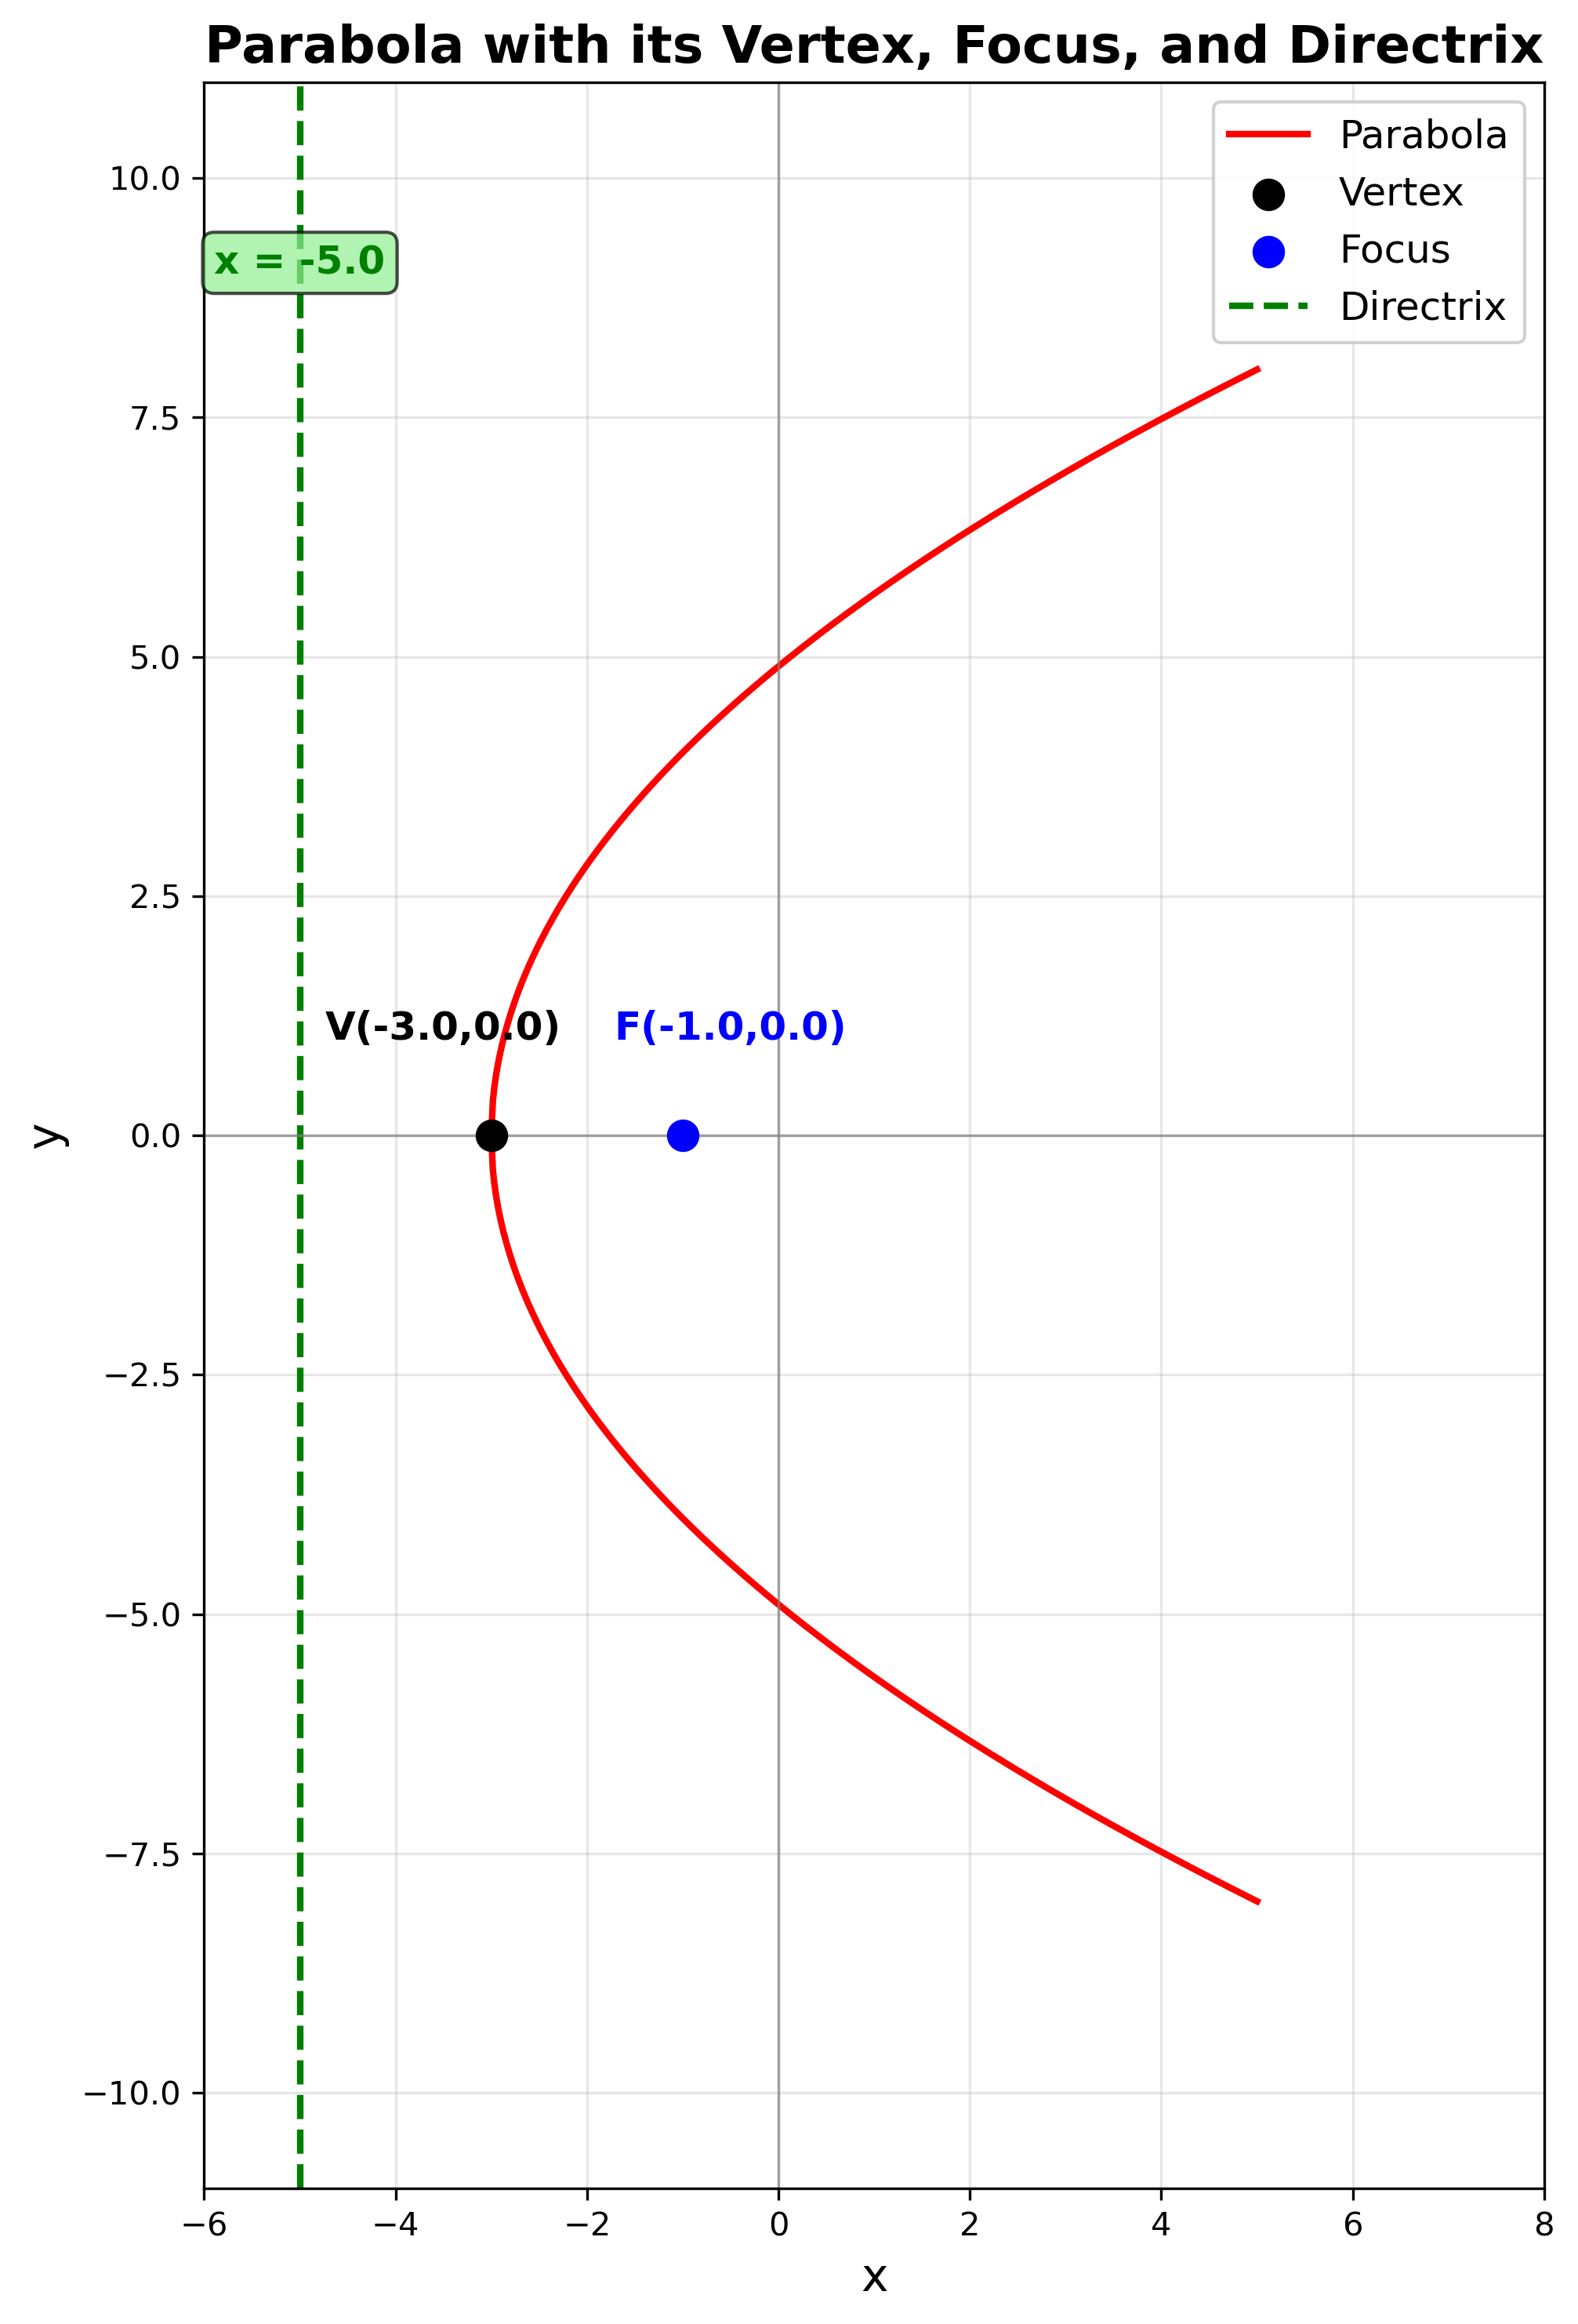
\includegraphics[width=\columnwidth, height=0.8\textheight, keepaspectratio]{figs/fig2.png}
    \label{fig:Beamer/figs/fig2.png}
\end{figure}
\end{frame}

\begin{frame}{Hyperbola}
\begin{figure}
   \centering
    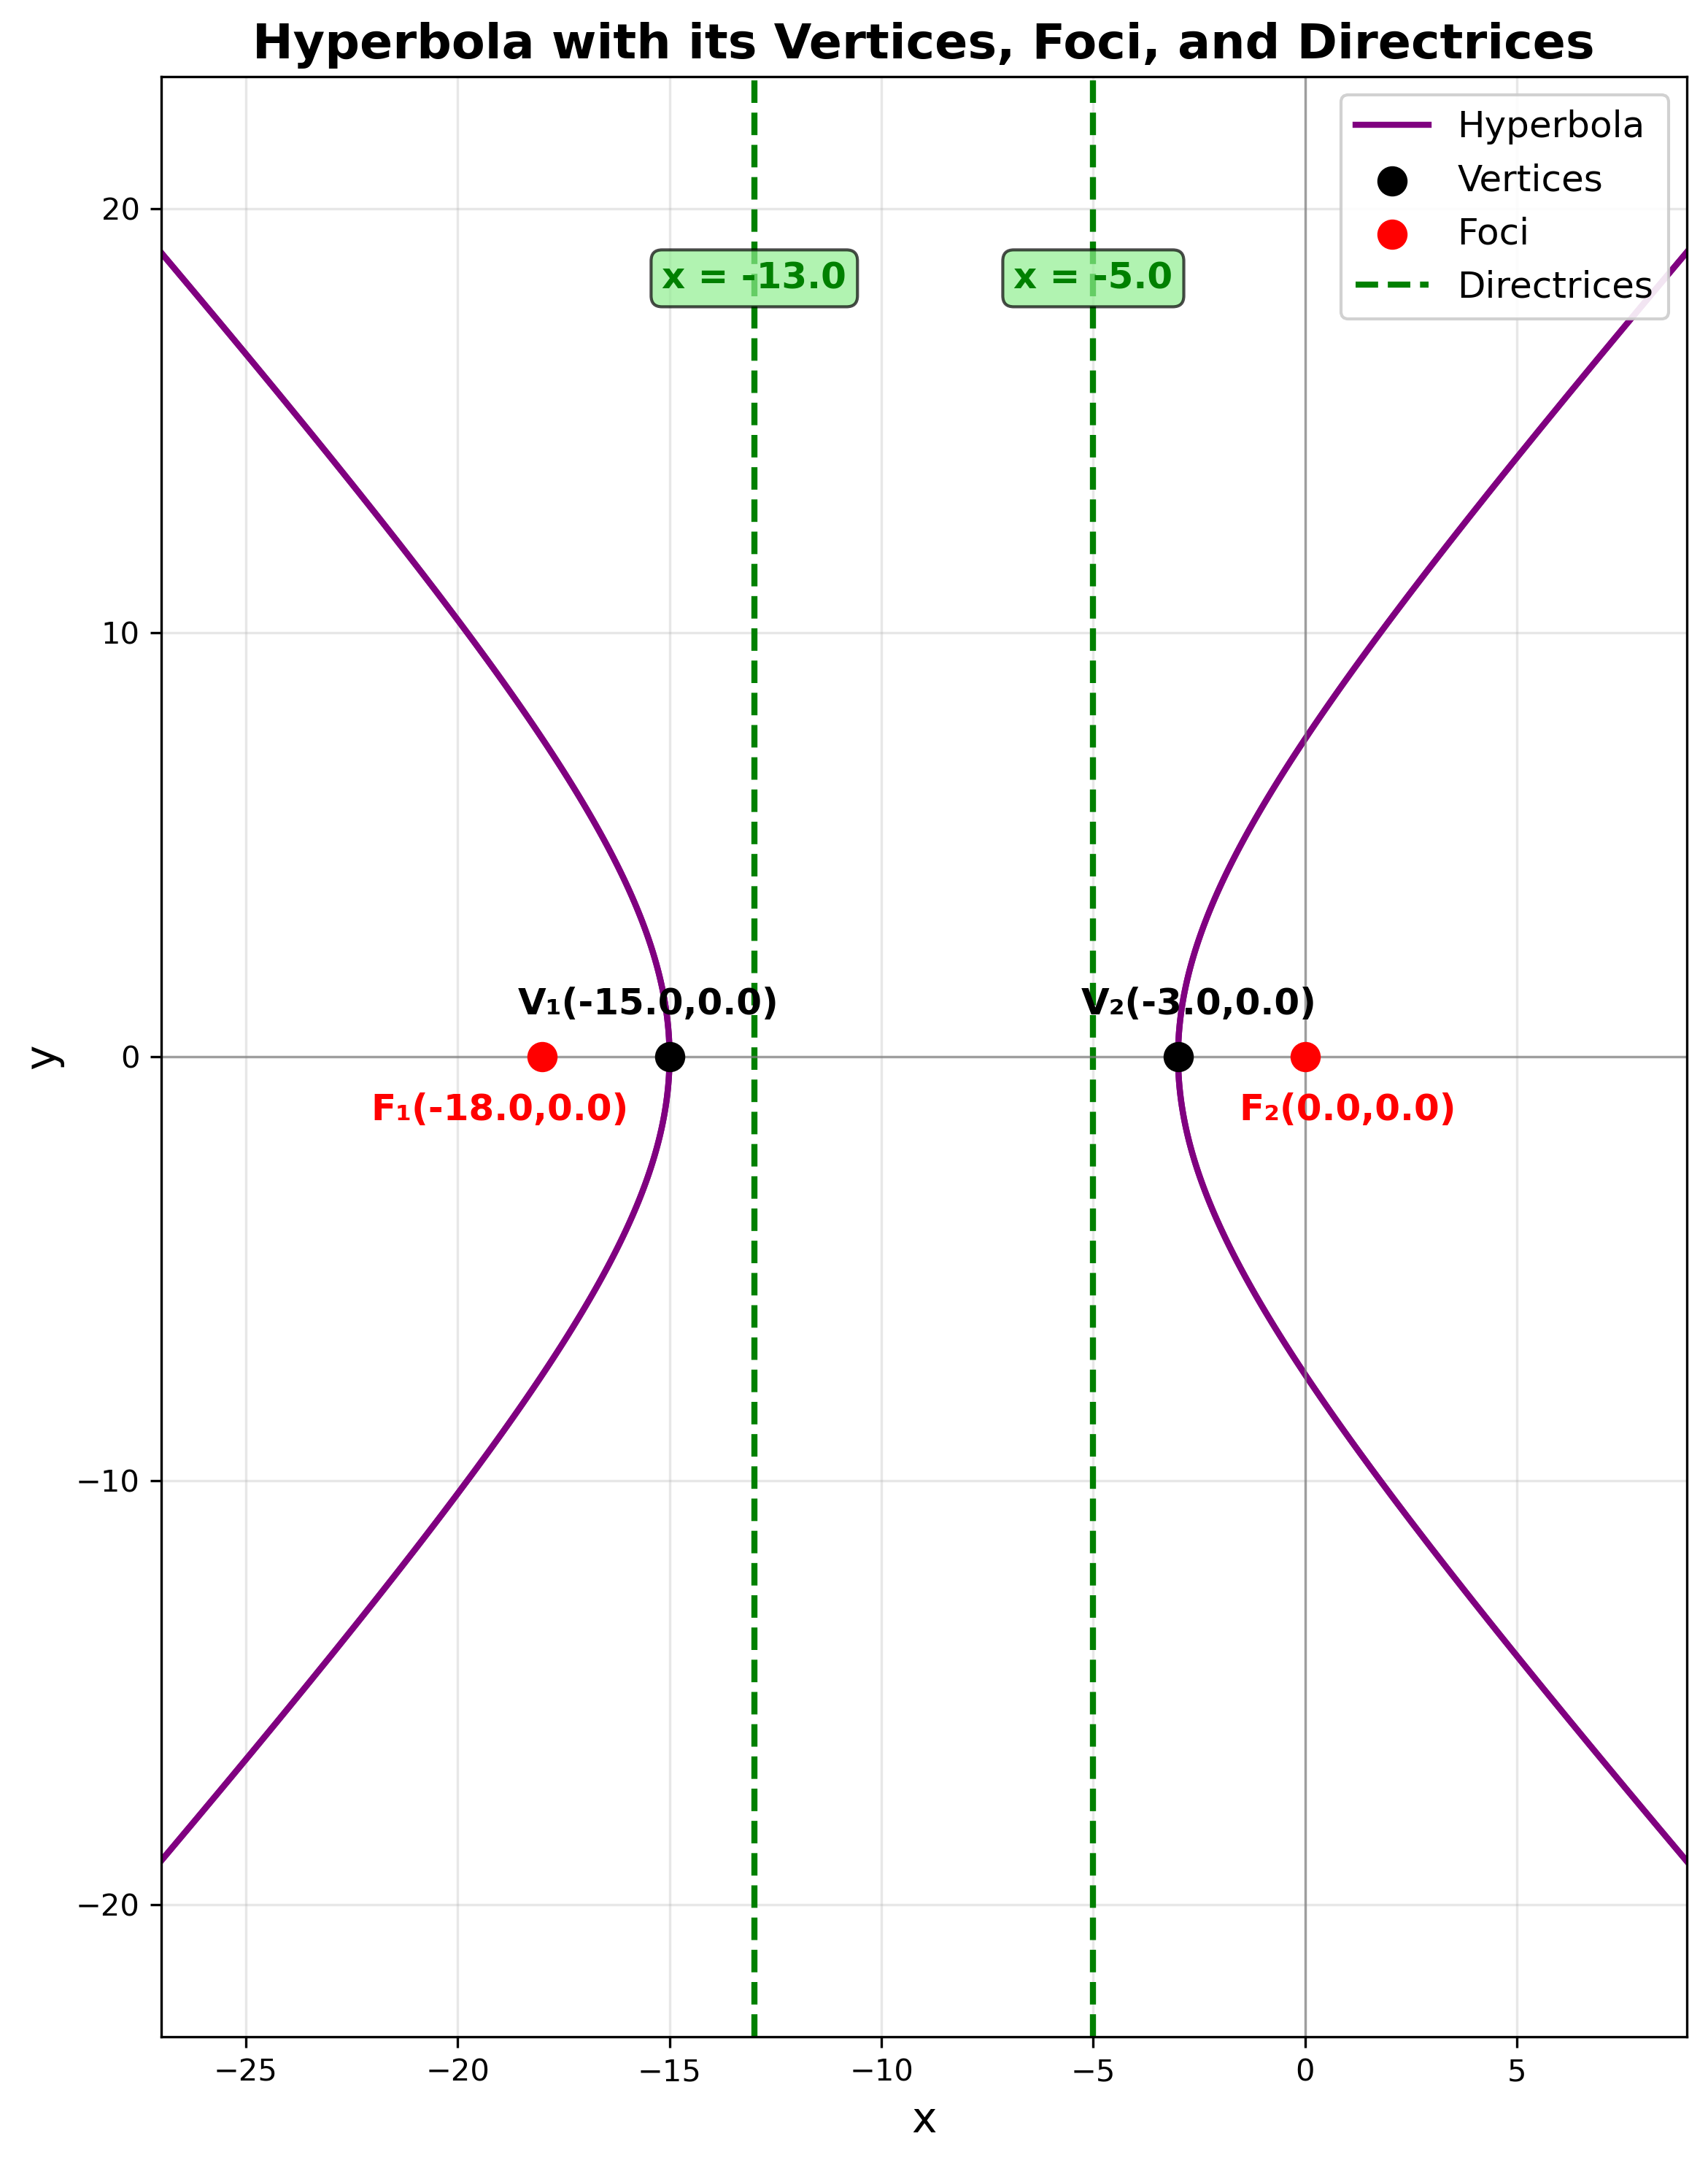
\includegraphics[width=\columnwidth, height=0.8\textheight, keepaspectratio]{figs/fig3.png}
    \label{fig:Beamer/figs/fig3.png}
\end{figure}
\end{frame}

\end{document}